\chapter{RDFS-Plus}
\label{ch9}

RDFS provides a very limited set of inference capabilities that, as we
have seen, have considerable utility in a Semantic Web setting for
merging information from multiple sources. In this chapter, we take the
first step toward the Web Ontology Language, OWL, in which more
elaborate constraints on how information is to be merged can be
specified. We have selected a particular set of OWL constructs to
present at this stage. This set was selected to satisfy a number of
goals:

\begin{itemize}
\item Pedagogically, these constructs constitute a gentle addition to the
constructs that are already familiar from RDFS, increasing the power of
the language without making a large conceptual leap from RDFS.

\item Practically, we have found that this set of OWL constructs has
considerable utility in the
information integration projects we have done. In fact, it is much
easier to find and describe case studies using RDFS plus this set of OWL
constructs than it is to find case studies that use RDFS by itself.

\item Computationally, this subset of OWL can be implemented using a wide
variety of inferencing technologies, lessening the dependency between
the Semantic Web and any particular technology.
\end{itemize}

For these reasons, we feel that this particular subset will have value
beyond the pedagogical value in this book. We call this subset of OWL
\emph{RDFS-Plus}, because we have seen a trend among vendors of Semantic Web tools
and Web applications designers for determining a subset of OWL that is
at the same time useful and can be implemented quickly. We have
identified this particular subset via an informal poll of cutting-edge
vendors, and from our own experience with early adopters of Semantic Web
technology.

Just as was the case for RDFS, RDFS-Plus is expressed entirely in RDF.
The only distinction is
that there are a number of resources, all in the namespace \texttt{owl:}. The
meaning of these resources is specified, as before, by the rules that
govern the inferences that can be made from them. As we did for RDFS, we
will specify the rules that govern the inferences using SPARQL CONSTRUCT
queries.

In the case of RDFS, we saw how the actions of an inference engine could
be used to combine various features of the schema language in novel
ways. This trend will continue for RDFS-Plus, but as you might expect,
the more constructs we have to begin with, the more opportunity we have
for useful and novel combinations.

\section{Inverse}

The names of many of the OWL constructs come from corresponding names in
mathematics. Despite their mathematical names, they also have a more
common, everyday interpretation. The idea \texttt{owl:inverseOf} is a prime
example; if a relationship---say, \texttt{hasParent}---is interesting enough to
mention in a model, then it's a good bet that another
relationship---say, \texttt{hasChild}---is also interesting. Because of the
evocative names \texttt{hasParent} and \texttt{hasChild}, you can guess the relationship
between them, but of course the computer can't. The OWL construct
\texttt{owl:inverseOf} makes the relationship between \texttt{hasParent} and \texttt{hasChild}
explicit, and describes precisely what it means.

In mathematics, the inverse of a function $f$ (usually written as $f^{-1}$) is
the function that satisfies the
property that if $f(x) = y$, then $f^-1(y) = x$. Similarly in OWL, the
inverse of a property is another property that reverses its direction.  This should not be confused with 
a semantic \textit{opposite};  you could imagine a model that describes two 
properties - \texttt{hasFriend} and \texttt{hasEnemy}.  These might be considered 'opposites', since 
by definition, a friend can't be an enemy and vice versa, but they are not mathematical inverses, in fact, far from it;
if I am your friend, it does not imply that you are my enemy.  OWL does not have a way to formally indicate this sort of 
relationship between properties. 

To be specific, we look at the meaning of \texttt{owl:inverseOf}. In OWL, as in
RDFS, the meaning of any construct is given by the inferences that can
be drawn from it. We can express the rule for owl:inverseOf in SPARQL as
follows:

\begin{lstlisting}
CONSTRUCT {?y ?q ?x}
WHERE {?p owl:inverseOf ?q .
       ?x ?p ?y . }
\end{lstlisting}

In the examples in the book, we have already seen a number of
possibilities for inverses, though we haven't used them so far. In our
Shakespeare examples, we have the triples

\begin{lstlisting}
lit:Shakespeare lit:wrote lit:Macbeth .
lit:Macbeth lit:setIn geo:Scotland .
\end{lstlisting}

If, in addition to these triples, we also state some inverses, such as:

\begin{lstlisting}
lit:wrote owl:inverseOf lit:writtenBy .
lit:settingFor owl:inverseOf lit:setIn .
\end{lstlisting}

then we can infer that

\begin{lstlisting}
lit:Macbeth lit:writtenBy lit:Shakespeare .
geo:Scotland lit:settingFor lit:Macbeth .
\end{lstlisting}

Although the meaning of \texttt{owl:inverseOf} is not difficult to describe, what
is the utility of such a construct in a modeling language? After all,
the effect of inverseOf can be achieved just as easily by writing the
query differently. For instance, if we want to know all the plays that
are \texttt{setIn} Scotland, we can use the inverse property \texttt{settingFor} in our
query pattern, such as

\begin{lstlisting}
{ geo:Scotland lit:settingfor ?play . }
\end{lstlisting}

Because of the semantics of the inverse property, this will give us all
plays that were setIn
Scotland.

But we could have avoided the use of the inverse property and simply
written the query as

\begin{lstlisting}
{ ?play lit:setIn geo:Scotland . }
\end{lstlisting}

We get the same answers, and we don't need an extra construct in the
modeling language.

While this is true, \texttt{owl:inverseOf} nevertheless does have considerable
utility in modeling, based on how it can interact with other modeling
constructs. In the next two challenges, we'll see how some earlier
challenges can be extended using inverses.

\begin{challenge}{continued from Challenge\protect\ref{chal:2}: Using SPARQL to Transform Hierarchical Data}

In Chapter~\ref{ch6} we saw a Challenge problem to use SPARQL to transform
hierarchical data. The original data was expressed using a variety of
properties like \texttt{hasSon}, \texttt{hasMother}, \texttt{hasDaughter}, and \texttt{hasFather}. The
response to the challenge involved a series of SPARQL queries to
transform e.g., \texttt{hasMother} into \texttt{hasParent}. The queries that accomplished
the transformations all had a very similar form, e.g.,

\begin{lstlisting}
CONSTRUCT {?s :hasParent ?o}
WHERE {?s :hasMother ?o}
\end{lstlisting}


The transformation that this query accomplishes can also be represented
in RDFS. This query says ``whenever a triple uses hasMother, infer a
similar triple with hasParent.'' This can be expressed in RDFS by
relating the two properties together with \texttt{subPropertyOf}, thus:

\begin{lstlisting}
:hasMother rdfs:subPropertyOf :hasParent .
\end{lstlisting}

When we combine this statement with the definition of \texttt{subPropertyOf}, we
see that we come to the same conclusions---from every triple that uses
hasMother we can infer a similar triple using hasParent.

Some of the queries included a bit of a twist on this pattern---for
example, one query rectified uses of
\texttt{hasSon} as follows:

\begin{lstlisting}
CONSTRUCT {?s :hasParent ?o}
WHERE {?o :hasSon ?s}
\end{lstlisting}



\begin{figure}
\centering
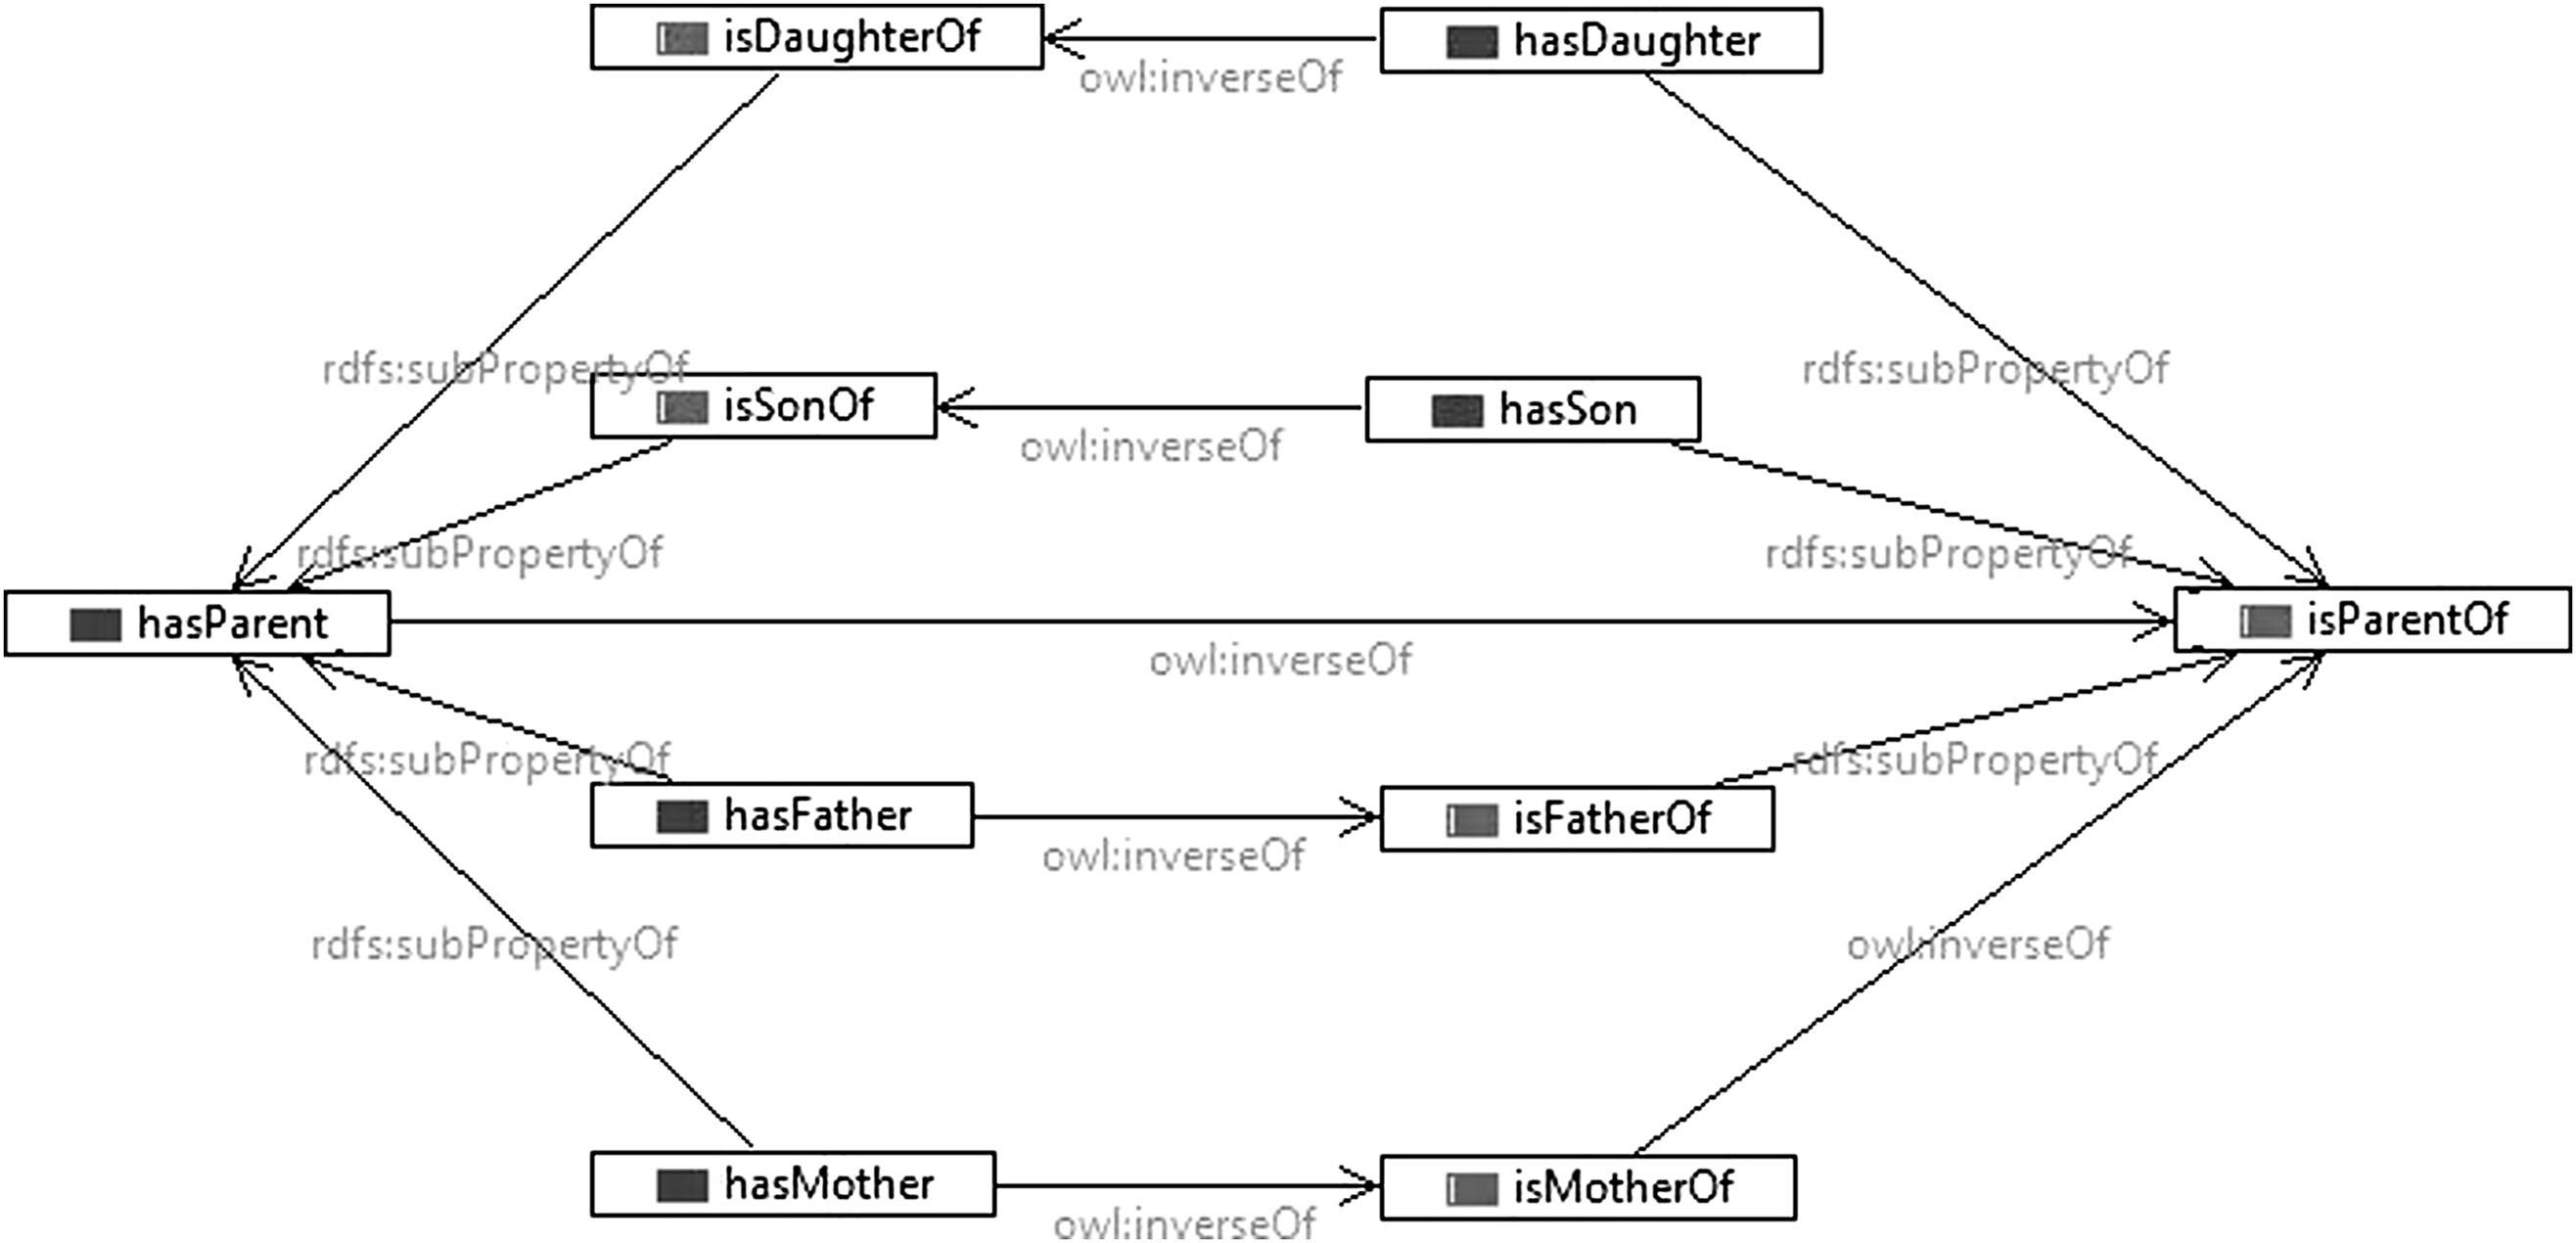
\includegraphics[width=5in]{media/ch9/f09-001.png}
\caption{Display of family relationships, and how they are connected. The figure shows only the
subPropertyOf relationships, not the inverseOf relationships.}
\label{fig:ch9.1}
\end{figure}




A simple \texttt{subPropertyOf} relationship can't capture the meaning of this
query, because the order of the subject and object are reversed. We
can't model this relationship in RDFS alone. But with the addition of
\texttt{inverseOf}, we can do it. We will need to introduce a new property that
is the inverse of \texttt{hasSon}. We'll call it \texttt{isSonOf}.

\begin{lstlisting}
:isSonOf owl:inverseOf :hasSon .
:isSonOf rdfs:subPropertyOf :hasParent .
\end{lstlisting}

Using the definition of \texttt{subPropertyOf} from RDFS, and the definition of
\texttt{inverseOf} from OWL, we get the same result as we did from the SPARQL
query---from each triple that use \texttt{hasSon}, we can infer a new triple
using \texttt{hasParent}, with the appropriate subject and object.

One advantage to representing these relationships in RDFS-Plus is that
all the relationships among these properties are represented in a single
model, and can even be displayed visually. If we define all the
variations of sons, daughters, parents, etc., we can see them in a
single display as shown in Figure~/ref{fig:ch9.1}.

This is a fairly common modeling pattern in RDFS-Plus, in which a
hierarchy of properties is specified, along with a corresponding
hierarchy of inverses.
\end{challenge}

\subsection{integrating data that do not want to be integrated}

In  Example~\ref{ex:ch8.1}, we had two properties, \texttt{borrows} and
\texttt{checkedOut}. We were able to combine them under a single property by
making them both \texttt{rdfs:subPropertyOf} the same parent property,
\texttt{hasPosession}. We were fortunate that the two sources of data happened to
link a \texttt{Patron} as the subject to a \texttt{Book} as the object (i.e., they had the
same domain and range). Suppose instead that the second source was an
index of books, and for each book there was a field specifying the
patron the book was \texttt{signedTo} (i.e., the domain and range are reversed).

\begin{challenge}{Merging inverse properties}

How can we merge \texttt{signedTo} and \texttt{borrows} in a way analogous to how we
merged \texttt{borrows} and
\texttt{checkedOut}, given that \texttt{signedTo} and \texttt{borrows} don't share good domains and
ranges?

\solution

The solution involves a simple use of \texttt{owl:inverseOf} to specify two
properties for which the domain and range do match, as required for the
merge. We define a new property---say, \texttt{signedOut}---as the inverse of
\texttt{signedTo}, as follows:

\begin{lstlisting}
:signedTo owl:inverseOf :signedOut.
\end{lstlisting}

Now we can use the original Property Union pattern to merge \texttt{signedOut}
and \texttt{borrows} into the single
\texttt{hasPossession} property:

\begin{lstlisting}
:signedOut rdfs:subPropertyOf :hasPossession .
:borrows rdfs:subPropertyOf :hasPossession .
\end{lstlisting}

So if we have some data expressed using \texttt{signedTo}, along with data
expressed with \texttt{borrows}, as follows:

\begin{lstlisting}
:Amit :borrows :MobyDick .
:Marie :borrows :Orlando .
:LeavesOfGrass :signedTo :Jim .
:WutheringHeights :signedTo :Yoshi .
\end{lstlisting}

then with the rule for \texttt{inverseOf}, we can infer the additional triples

\begin{lstlisting}
* :Jim :signedOut :LeavesOfGrass.
* :Yoshi :signedOut :WutheringHeights.
\end{lstlisting}

and with \texttt{subPropertyOf}, we have

\begin{lstlisting}
* :Amit :hasPossession :MobyDick.
* :Marie :hasPossession :Orlando.
* :Jim :hasPossession :LeavesOfGrass.
* :Yoshi :hasPossession :WutheringHeights.
\end{lstlisting}

as desired.

\solution (alternative)

There is a certain asymmetry in this solution; the choice to specify an
inverse for \texttt{signedTo} rather than for \texttt{hasPossession} was somewhat
arbitrary. Another solution that also uses \texttt{owl:inverseOf} and
\texttt{rdfs:subPropertyOf} and is just as viable as the first is the following:

\begin{lstlisting}
:signedTo :rdfs:subPropertyOf :possessedBy .
:borrows rdfs:subPropertyOf :hasPossession .
:possessedBy owl:inverseOf :hasPossession .
\end{lstlisting}

These statements use the same rules for \texttt{owl:inverseOf} and
\texttt{rdfs:subPropertyOf} but in a different order, resulting in the same
\texttt{hasPossession} triples. Which solution is better in what situations? How
can we tell which to use?



\begin{figure}
\centering
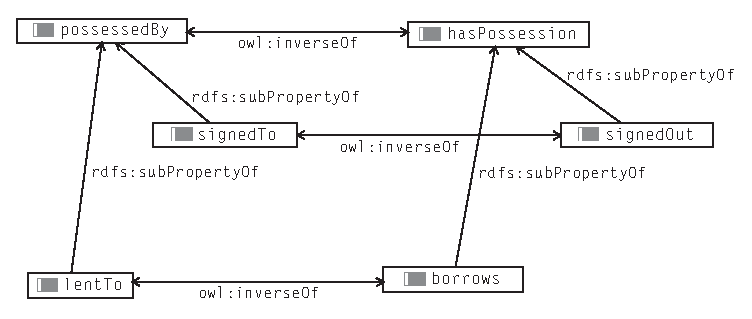
\includegraphics[width=5in]{media/ch9/f09-002.eps}
\caption{Systematic combination of inverseOf and subPropertyOf.}
\label{fig:ch9.2}
\end{figure}


If all we were concerned with was making sure that the inferences about
\texttt{hasPossession} will be supported, then there would be no reason to prefer
one solution over the other. But modeling in the Semantic Web is not
just about supporting desired inferences but also about supporting
reuse. What if someone else
wants to use this model in a slightly different way? A future query is
just as likely to be interested in \texttt{hasPossession} as \texttt{possessedBy}.
Furthermore, we might in the future wish to combine \texttt{hasPossession} (or
\texttt{possessedBy}) with another property. For this reason, one might choose to
use both solutions together by using both \texttt{inverseOf} and \texttt{subPropertyOf} in
a systematic way---that is, by specifying inverses for every property,
regardless of the subPropertyOf level. In this case, this results in

\begin{lstlisting}
:signedTo owl:inverseOf :signedOut.
:signedTo rdfs:subPropertyOf :possessedBy.
:signedOut rdfs:subPropertyOf :hasPossession.
:lentTo owl:inverseOf :borrows.
:lentTo rdfs:subPropertyOf :possessedBy.
:borrows rdfs:subPropertyOf :hasPossession.
:possessedBy owl:inverseOf :hasPossession.
\end{lstlisting}

The systematicity of this structure can be more readily seen in Figure~\ref{Figch9.2}. 
The attentive reader might have one more concern about the
systematicity of Figure~\ref{Figch9.2}---in particular, the selection of which
properties are the subject of \texttt{owl:inverseOf} and which are the object (in
the diagram, which ones go on the left or on the right of the diagram)
is arbitrary. Shouldn't there be three more \texttt{owl:inverseOf} triples,
pointing from right to left? Indeed, there should be, but there is no
need to assert these triples, as we shall see in the next challenge.
\end{challenge}


\subsection{Using the modeling language to extend the modeling language}

It is not unusual for beginning modelers to look at the list of
constructs defined in OWL and say, ``There is a feature of the OWL
language I would like to use that is very similar to the ones that are
included. Why did they leave it out? I would prefer to build my model
using a different set of primitives.'' In many cases, the extra language
feature that they desire is actually already supported by OWL as a
combination of other features. It is a simple matter of using these
features in combination.

\begin{challenge}{Superclasses}

For example, RDFS allows you to specify that one class is a subClassOf
another, but you might like to think of it the other way around (perhaps
because of the structure of some legacy data you want to work with) and
specify that something is superClassOf something else. That is, you want
the parent class to be the subject of all the definitional triples.
Using your own namespace myowl: for this desired relation, you would
like to have the triples look like this:

\begin{lstlisting}
:Food myowl:superClassOf :BakedGood; 
      myowl:superClassOf :Confectionary;
      myowl:superClassOf :PackagedFood;
      myowl:superClassOf :PreparedFood;
      myowl:superClassOf :ProcessedFood.
\end{lstlisting}

If we instead use \texttt{rdfs:subClassOf}, all the triples go the other way
around; Food will be the object of each triple, and all the types of
Food will be the subjects.

Since OWL does not provide a superClassOf resource (or to speak more
correctly, OWL does not define any inference rules that will provide any
semantics for a superClassOf resource), what can we do?

\solution

What do we want \texttt{myowl:superClassOf} to mean? For every triple of the form

\begin{lstlisting}
?P myowl:superClassOf ?Q.
\end{lstlisting}

we want to be able to infer that

\begin{lstlisting}
* ?Q rdfs:subClassOf ?P.
\end{lstlisting}

This can be accomplished simply by declaring an inverse

\begin{lstlisting}
myowl:superClassOf owl:inverseOf rdfs:subClassOf.
\end{lstlisting}

It is a simple application of the rule for \texttt{owl:inverseOf} to see that
this accomplishes the desired effect. Nevertheless, this is not a
solution that many beginning modelers think of. It seems to them that
they have no right to modify or extend the meaning of the OWL language
or to make statements about the OWL and RDFS resources (like
\texttt{rdfs:subClassOf}). But remember the AAA slogan of RDF: Anyone can say
Anything about Any topic. In particular, a modeler can say things about
the resources defined in the standard.

In fact, we can take this slogan so far as to allow a modeler to say

\begin{lstlisting}
rdfs:subClassOf owl:inverseOf rdfs:superClassOf.
\end{lstlisting}

This differs from the previous triple in that the subject is a resource
in the (standard) RDFS namespace. The AAA slogan allows a modeler to say
this,  and indeed, there is nothing in the standards that will prevent
it. But this practice is problematic; as we saw in Chapter~\ref{ch5}, it is normally possible to de-reference 
an HTTP URI to learn more about a resource.  Since only the W3C can add new content to the 
web servers at the RDFS namespace, any attempt to de-reference rdfs:superClassOf will fail to return any information. 
Another problem with this practice is that  a reference to a resource in the RDFS namespace 
suggests to human readers of the model that this resource is part of
the RDFS standard (which it is not). Since one purpose of a model is to communicate to
other human beings, it is generally not a good idea to make statements
that are likely to be misleading.   The AAA slogan is like free speech; just because you are 
allowed to say something, doesn't mean that you should. 
\end{challenge}

\subsection{Symmetric  properties in queries}

Consider a simple model about the marriage of Shakespeare---a model with
only one triple.

\begin{lstlisting}
bio:AnneHathaway bio:married lit:Shakespeare.
\end{lstlisting}

If we were to query this with the SPARQL query

\begin{lstlisting}
SELECT ?who
WHERE {?lit:Shakespeare bio:married ?who}
\end{lstlisting}

We would get no answer---Shakespeare married no one, despite our
intuition that marriage is a two-way street. We would like to express
this part of our understanding of how marriage works in a model.

\begin{challenge}{The marriage of Shakespeare}

How can we infer marriages in the reverse direction from which they are
asserted?

\solution

We could do this by simply declaring \texttt{bio:married} to be its own inverse,
thus:

\begin{lstlisting}
bio:married owl:inverseOf bio:married.
\end{lstlisting}

Now any triple that used \texttt{bio:married} would automatically be inferred to
hold in the other direction. In particular, if we asserted

\begin{lstlisting}
bio:AnneHathaway bio:married lit:Shakespeare.
\end{lstlisting}

we could infer that

\begin{lstlisting}
* lit:Shakespeare bio:married bio:AnneHathaway.
\end{lstlisting}

This pattern of self-inverses is so common that it has been built into
OWL using a special construct called
\texttt{owl:SymmetricProperty}.

\subsection{Symmetric Properties}

\texttt{owl:inverseOf} relates one property to another. The special case in which
these two properties are the same (as was the case for \texttt{bio:married} for
the Shakespeare example) is common enough that the OWL language provides
a special name for it: \texttt{owl:SymmetricProperty}. Unlike \texttt{owl:inverseOf},
which is a property that relates two other properties,
\texttt{owl:SymmetricProperty} is just an aspect of a single property and is
expressed in OWL as a Class. We express that a property is symmetric in
the same way as we express membership in any class---in other words:

\begin{lstlisting}
:P a owl:SymmetricProperty.
\end{lstlisting}

As usual, we express the meaning of this statement in SPARQL:

\begin{lstlisting}
CONSTRUCT {?p owl:inverseOf ?p. }
WHERE {?p a owl:SymmetricProperty . }
\end{lstlisting}

So in the case of the marriage of Shakespeare, we can simply assert that

\begin{lstlisting}
bio:married a owl:SymmetricProperty.
\end{lstlisting}
\end{challenge}


\begin{figure}
\centering
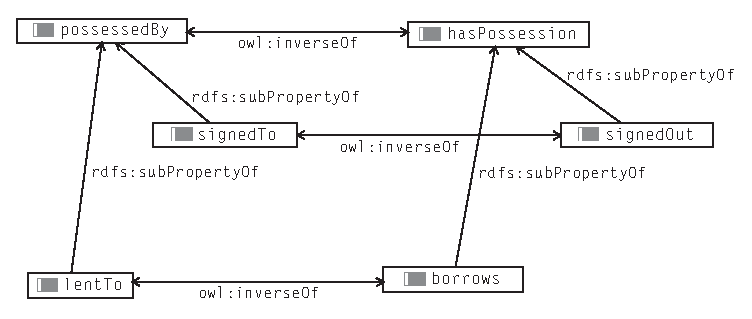
\includegraphics[width=5in]{media/ch9/f09-003.eps}
\caption{Systematic combination of inverseOf and subPropertyOf. Contrast this
with Figure~\ref{fig:ch9.2}, with one- directional inverses.
}
\label{fig:ch9.3}
\end{figure}



\subsection{Using OWL to extend OWL}

As we describe more and more of the power of the OWL modeling language,
there will be more and more opportunities to define at least some
aspects of a new construct in terms of previously defined constructs. We
can use this method to streamline our presentation of the OWL language.
We have seen a need for this already in figure Figure~\ref{fig:ch9.2}, in which all
of our inverses are expressed in one direction but we really need to
have them go both ways, as shown in Figure~\ref{fig:ch9.3}.

We asserted the triples from left to right---namely:

\begin{lstlisting}
:possessedBy owl:inverseOf :hasPossession.
:signedTo owl:inverseOf :signedOut.
:lentTo owl:inverseOf :borrows.
\end{lstlisting}

But we would like to be able to infer the triples from right to
left---namely:

\begin{lstlisting}
:hasPossession owl:inverseOf :possessedBy.
:signedOut owl:inverseOf :signedTo.
:borrows owl:inverseOf :lentTo.
\end{lstlisting}

\begin{challenge}{Modeling self-inverses}

How can we infer all of these triples without having to assert them?

\solution

Since we want \texttt{owl:inverseOf} to work in both directions, this can be done
easily by asserting that
\texttt{owl:inverseOf} is its own inverse, thus:

\begin{lstlisting}
owl:inverseOf owl:inverseOf owl:inverseOf .
\end{lstlisting}



You might have done a double take when you read that \texttt{owl:inverseOf} is
its own inverse. Fortunately, we now have a more readable and somewhat
more understandable way to say this---namely that it is symmetric:

\begin{lstlisting}
owl:inverseOf a owl:SymmetricProperty.
\end{lstlisting}

In either case, we get the inferences we desire for Figure\ref{fig:ch9.3}, in which
the inverses point both ways. This also means that all the inferences in
both directions will always be found.

\subsection{TRANSITIVITY}

In mathematics, a relation R is said to be transitive if $R(a,b)$ and
$R(b,c)$ implies $R(a,c)$. The same idea is used for the OWL construct
\texttt{owl:TransitiveProperty}. Just like \texttt{owl:SymmetricProperty},
\texttt{owl:TransitiveProperty} is a class of properties, so a model can assert
that a property is a member of the class

\begin{lstlisting}
:P a owl:TransitiveProperty.
\end{lstlisting}

The meaning of this is given by a somewhat more elaborate rule than we
have seen so far in this chapter.

\begin{lstlisting}
CONSTRUCT {?x ?p ?z .}
WHERE {?x ?p ?y .
       ?y ?p ?z .
       ?p a owl:TransitiveProperty . }
\end{lstlisting}

Notice that there is no need for even more elaborate rules like

\begin{lstlisting}
CONSTRUCT {?a ?p ?d .}
WHERE {?a ?p ?b .
       ?b ?p ?c .
       ?c ?p ?d . }
\end{lstlisting}

since this conclusion can be reached by applying the simple rule over
and over again.

Some typical examples of transitive properties include
ancestor/descendant (if Victoria is an ancestor of Edward, and Edward is
an ancestor of Elizabeth, then Victoria is an ancestor of Elizabeth) and
geographical containment (if Osaka is in Japan, and Japan is in Asia,
then Osaka is in Asia).

\subsection{Relating parents to ancestors}

A model of genealogy will typically include notions of parents as well
as ancestors, and we'd like them to fit together. But parents are not
transitive (my parents' parents are not my parents), whereas ancestors
are.

\begin{challenge}{Transitive superproperties}
\label{chal:17}

How can we allow a model to maintain consistent ancestry information,
given parentage information?

\solution

Start by defining the parent property to be a subPropertyOf the ancestor
property, thus:

\begin{lstlisting}
:hasParent rdfs:subPropertyOf :hasAncestor.
\end{lstlisting}

Then declare ancestor (only) to be a transitive property:

\begin{lstlisting}
:hasAncestor a owl:TransitiveProperty.
\end{lstlisting}

Let's see how this works on some examples.

\begin{lstlisting}
:Alexia :hasParent :WillemAlexander.
:WillemAlexander :hasParent :Beatrix.
:Beatrix :hasParent :Wilhelmina.
\end{lstlisting}

Because of the \texttt{subPropertyOf} relation between \texttt{hasParent} and \texttt{hasAncestor}
and the fact that
\texttt{hasAncestor} is a \texttt{TransitiveProperty}, we can infer that

\begin{lstlisting}
:Alexia :hasAncestor :WillemAlexander.
:WillemAlexander :hasAncestor :Beatrix.
:Alexia :hasAncestor :Beatrix.
:WillemAlexander :hasAncestor :Wilhelmina.
:Alexia :hasAncestor :Wilhelmina.
\end{lstlisting}

Information about the heritage is integrated, regardless of whether it
originated with \texttt{hasParent} or \texttt{hasAncestor}. Information about hasParent,
on the other hand, is only available as it was directly asserted because
it was not declared to be transitive. The results of this inference are
shown in Figure 8.4.
\end{challenge}

\begin{figure}
\centering
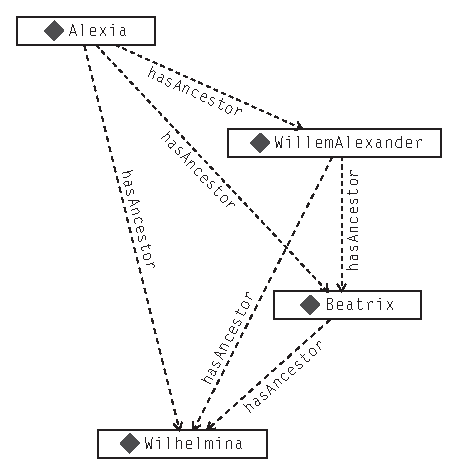
\includegraphics[width=5in]{media/ch9/f09-004.eps}
\caption{Inferences from transitive properties.}
\label{fig:ch9.4}
\end{figure}



\subsection{Layers of relationships}

Sometimes it can be somewhat controversial whether a property is
transitive or not. For instance, the relationship that is often
expressed by the words ``part of'' in English is sometimes transitive (a
piston is part of the engine, and the engine is part of the car; is the
piston part of the car?) and sometimes not (Mick Jagger's thumb is part
of Mick Jagger, and Mick Jagger is part of the Rolling Stones; is Mick
Jagger's thumb part of the Rolling Stones?). In the spirit of
anticipating possible uses of a model, it is worthwhile to support both
points of view whenever there is any chance that controversy might
arise.

\begin{challenge}{Managing transitive relations alongside non-transitive ones}
\label{chal:18}
How can we simultaneously maintain transitive and nontransitive versions
of the \texttt{partOf} information?

\solution

We can define two versions of the \texttt{partOf} property in different
namespaces (or with different names) with one a \texttt{subPropertyOf} the other,
and with the superproperty declared as transitive:

\begin{lstlisting}
dm:partOf rdfs:subPropertyOf gm:partOf.
gm:partOf a owl:TransitiveProperty.
\end{lstlisting}


\begin{figure}
\centering
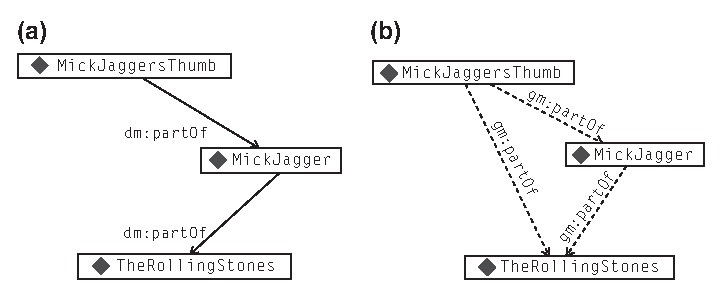
\includegraphics[width=5in]{media/ch9/f09-005.eps}
\caption{Different interpretations of partOf.}
\label{fig:ch8.5}
\end{figure}



Depending on which interpretation of \texttt{partOf} any particular application
needs, it can query the appropriate property. For those who prefer to
think that Mick Jagger's thumb is not part of the Rolling Stones, the
original \texttt{dm:partOf} property is useful. For those who instead consider
that Mick Jagger's thumb is part of the Rolling Stones, the transitive
superproperty \texttt{gm:partOf} is appropriate (see Figure\label{fig:ch8.5})
\end{challenge}

\section{Managing networks of dependencies}

The same modeling patterns we have been using to manage relationships
(like ancestry) or set containment (like part of) can be used just as
well in a very different setting---namely, to manage networks of
dependencies. In the series of challenges that follow, we will see how
the familiar constructs of \texttt{rdfs:subPropertyOf}, \texttt{owl:inverseOf}, and
\texttt{owl:TransitiveProperty} can be combined in novel ways to model important
aspects of such networks.

A common application of this idea is in workflow management. In a
complex working situation, a variety of tasks must be repeatedly
performed in a set sequence. The idea of workflow management is that the
sequence can be represented explicitly and the progress of each task
tracked in that sequence. Why would someone want to model workflow in a
Semantic Web? The answer is for the same reason one wants to put
anything on the Web: so that parts of the workflow can be shared with
others, encouraging reuse, review, and publication of work fragments.

Real workflow specifications are far too detailed to serve as examples
in a book, so we will use a simple example to show how it works. Let's
make some ice cream, using the following recipe:


\begin{quote}
Slice a vanilla bean lengthwise, and scrape the contents into 1 cup of
heavy cream. Bring the mixture to a simmer, but do not boil. While the
cream is heating, separate three eggs. Add 1/2 cup white sugar to the
eggs and beat until fluffy. Gradually add the warm cream, beating
constantly. Return the custard mixture to medium heat, and cook until
mixture leaves a heavy coat on the back of a spatula. Chill well. Combine custard with 1 cup whole milk, and turn in ice cream freezer according to manufacturer's instructions.
\end{quote}



\begin{figure}
\centering
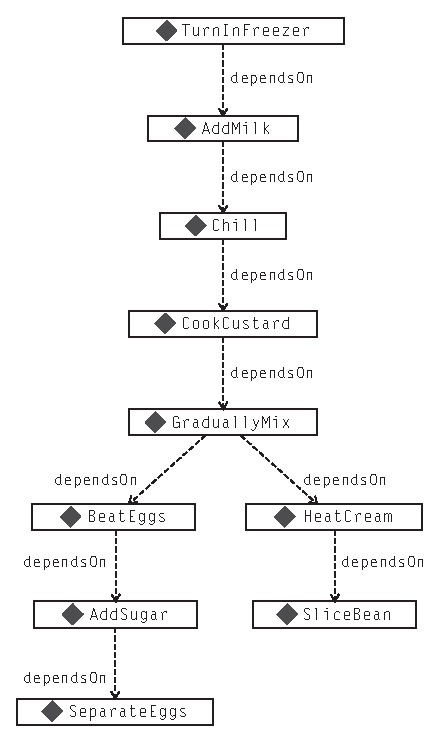
\includegraphics[width=5in]{media/ch9/f09-006.eps}
\caption{Dependencies for homemade ice cream.}
\label{fig:ch9.6}
\end{figure}


First, let's use a property \texttt{dependsOn} to represent the dependencies
between the steps and define its inverse enables, since each step
enables the next in the correct execution of the workflow:

\begin{lstlisting}
:dependsOn owl:inverseOf :enables.
\end{lstlisting}

Now we can define the dependency structure of the recipe steps:

\begin{lstlisting}
:SliceBean :enables :HeatCream.
:SeparateEggs :enables :AddSugar.
:AddSugar :enables :BeatEggs
:BeatEggs :enables :GraduallyMix.
:HeatCream :enables :GraduallyMix.
:GraduallyMix :enables :CookCustard.
:CookCustard :enables :Chill.
:Chill :enables :AddMilk.
:AddMilk :enables :TurnInFreezer.
\end{lstlisting}

Because of the \texttt{inverseOf}, we can view these steps either in enabling
order as asserted or in dependency order, as shown in Figure\ref{fig:ch9.6}.

\begin{challenge}{Managing an ice-cream recipe}

For any particular step in the process, we might want to know all the
steps it depends on or all the steps that depend on it. How can we do
this, using the patterns we already know?

\solution

We can use the \texttt{subPropertyOf}/\texttt{TransitiveProperty} pattern for each of
dependsOn and
enables as follows:

\begin{figure}
\centering
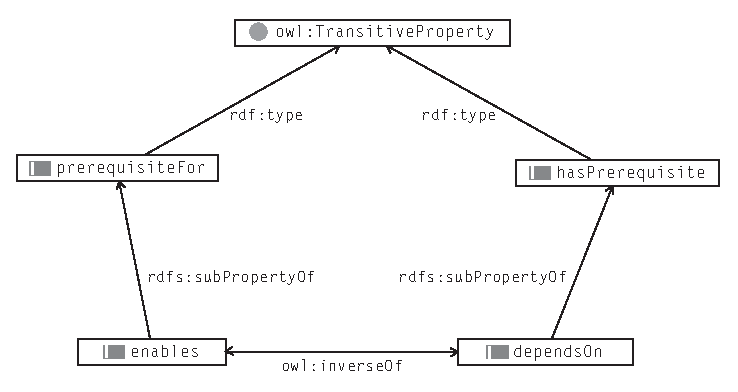
\includegraphics[width=5in]{media/ch9/f09-007.eps}
\caption{Transitive properties hasPrerequisite and prerequisiteFor defined in
terms of dependsOn and enables.
}
\label{fig:ch9.7}
\end{figure}



These relationships can be seen graphically in Figure\ref{fig:ch9.7}

From these triples, for instance, we can infer that GraduallyMix has
five prerequisites---
namely:

\begin{lstlisting}
* :GraduallyMix :hasPrerequisite :AddSugar ;
*               :hasPrerequisite :SeparateEggs ;
*               :hasPrerequisite :SliceBean ;
*               :hasPrerequisite :HeatCream ;
*               :hasPrerequisite :BeatEggs .
\end{lstlisting}
\end{challenge}


\begin{challenge}{Managing workflow}

In a more realistic workflow management setting, we wouldn't just be
managing a single process (corresponding to a single recipe). We would
be managing several processes that interact in complex ways. We could
even lose track of which steps are in the same procedure. Is there a way
to find out, given a particular step, what the other steps in the same
process are? In our recipe example, can we model the relationship
between steps so that we can connect steps in the same recipe together?

\solution

First, we combine together both of our fundamental relationships
(\texttt{enables} and \texttt{dependsOn}) as common \texttt{subPropertyOf} a single unifying
property (\texttt{neighborStep}). We then, in turn, make that a \texttt{subPropertyOf} of
a transitive property (\texttt{inSameRecipe}), shown here in Turtle and in Figure~\ref{fig:ch9.8}(a).

\begin{lstlisting}
:dependsOn rdfs:subPropertyOf :neighborStep.
:enables rdfs:subPropertyOf :neighborStep.
:neighborStep rdfs:subPropertyOf :inSameRecipe.
:inSameRecipe a owl:TransitiveProperty.
\end{lstlisting}

What inferences can we draw from these triples for the instance
\texttt{GraduallyMix}? Any directly related step (related by either \texttt{dependsOn} or
\texttt{enables}) becomes a \texttt{neighborStep}, and any combination of neighbors is
rolled up with \texttt{inSameRecipe}. A few selected inferences are shown here:

\begin{lstlisting}
:GraduallyMix :neighborStep :BeatEggs ;
              :neighborStep :HeatCream ;
              :neighborStep :CookCustard .
:CookCustard  :neighborStep :Chill ;
              :neighborStep :GraduallyMix .
:GraduallyMix :inSameRecipe :BeatEggs ;
              :inSameRecipe :HeatCream ;
              :inSameRecipe :CookCustard .
:CookCustard  :inSameRecipe :Chill ;
              :inSameRecipe :GraduallyMix .
        ...
:GraduallyMix :inSameRecipe :AddMilk ;
              :inSameRecipe :CookCustard ;
              :inSameRecipe :TurnInFreezer ;
              :inSameRecipe :AddSugar ;
              :inSameRecipe :SeparateEggs ;
              :inSameRecipe :SliceBean ;
              :inSameRecipe :HeatCream ;
              :inSameRecipe :GraduallyMix ;
              :inSameRecipe :Chill ;
              :inSameRecipe :BeatEggs .
\end{lstlisting}



\begin{figure}
\centering
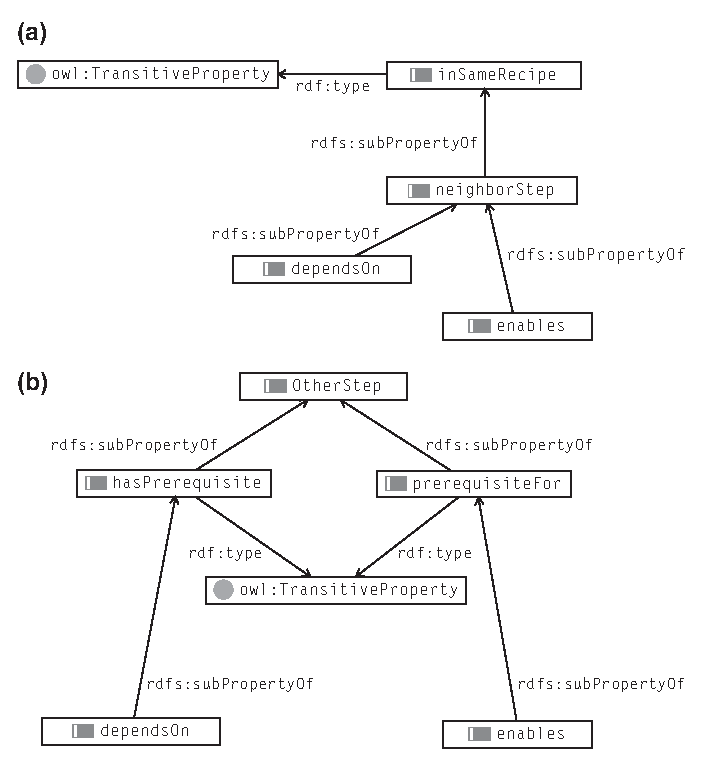
\includegraphics[width=5in]{media/ch9/f09-008.eps}
\caption{Contrast patterns for inSameRecipe (includes self) and otherStep
(excludes self). Both patterns work from the same input properties
dependsOn and enables but yield different results.}
\label{fig:ch9.8}
\end{figure}



All the steps in this recipe have been gathered up with \texttt{inSameRecipe}, as
desired. In fact, any two steps in this recipe will be related to one
another by \texttt{inSameRecipe}, including relating each step to itself. In
particular, the triple

\begin{lstlisting}
:GraduallyMix :inSameRecipe :GraduallyMix.
\end{lstlisting}

has been inferred. Although this is, strictly speaking, correct (after
all, indeed \texttt{GraduallyMix} is in the same recipe as \texttt{GraduallyMix}), it
might not be what we actually wanted to know.
\end{challenge}


\begin{challenge}{Finding other steps}

How can we define a property that will relate a recipe step only to the
other steps in the same recipe?

\solution

Earlier we defined two properties, \texttt{hasPrerequisite} and \texttt{prerequisiteFor},
one looking ``downstream'' along the dependencies and one looking
``upstream.''

\begin{lstlisting}
:dependsOn rdfs:subPropertyOf :hasPrerequisite.
:hasPrerequisite a owl:TransitiveProperty.
:enables rdfs:subPropertyOf :prerequisiteFor.
:prerequisiteFor a owl:TransitiveProperty.
\end{lstlisting}

If we join these two together under a common superproperty that is not
transitive, we get the following:

\begin{lstlisting}
:hasPrerequisite rdfs:subPropertyOf :otherStep .
:prerequisiteFor rdfs:subPropertyOf :otherStep .
\end{lstlisting}

These relationships are shown diagrammatically in Figure\ref{fig:ch9.8}(b).

We track the inferences separately for each property. For
\texttt{hasPrerequisite}, we have already seen that we can infer the following:

\begin{lstlisting}
:GraduallyMix :hasPrerequisite :AddSugar ;
              :hasPrerequisite :SeparateEggs ;
              :hasPrerequisite :SliceBean ;
              :hasPrerequisite :HeatCream ;
              :hasPrerequisite :BeatEggs .
\end{lstlisting}

For \texttt{prerequisiteFor}, we get the following inferences:

\begin{lstlisting}
:GraduallyMix :prerequisiteFor :AddMilk ;
              :prerequisiteFor :CookCustard ;
              :prerequisiteFor :TurnInFreezer ;
              :prerequisiteFor :Chill .
\end{lstlisting}

Now, for otherStep, we get the combination of these two. Notice that
neither list includes Gradually
Mix itself, so it does not appear in this list either.

\begin{lstlisting}
:GraduallyMix :otherStep :AddMilk ;
              :otherStep :CookCustard ;
              :otherStep :TurnInFreezer ;
              :otherStep :AddSugar ;
              :otherStep :SeparateEggs ;
              :otherStep :SliceBean ;
              :otherStep :HeatCream ;
              :otherStep :Chill ;
              :otherStep :BeatEggs .
\end{lstlisting}

Figure\ref{fig:ch9.8} shows the two patterns. For \texttt{inSameRecipe}, we have a single
transitive property at the top of a subPropertyOf tree; both primitive
properties (\texttt{enables} and \texttt{dependsOn}) are brought together, and any
combinations of the resulting property (\texttt{neighborStep}) are chained
together as a TransitiveProperty (\texttt{inSameRecipe}). For otherStep, the
top-level property itself is not transitive but is a simple combination
(via two subPropertyOf links) of two transitive properties
(\texttt{hasPrerequisite} and \texttt{prerequisiteFor}). Inference for each of these
transitive properties is done separately from the other, and the results
combined (without any more transitive interaction). Hence, for
\texttt{inSameRecipe}, the reflexive triples like

\begin{lstlisting}
:GraduallyMix :inSameRecipe :GraduallyMix
\end{lstlisting}

are included, whereas for \texttt{otherStep}, they are not.

Another ramification of the difference between these two models has to
do with whether or not they can ``turn the corner'' in Figure~\ref{fig:ch9.6} and
determine a relationship between, e.g., \texttt{BeatEggs} and \texttt{HeatCream}. The
transitive structure of \texttt{inSameRecipe} allows this to happen, whereas for
\texttt{otherStep} it does not; that is, we can infer

\begin{lstlisting}
\begin{lstlisting}
:BeatEggs :inSameRecipe :HeatCream
end{lstlisting}
but not
:BeatEggs :otherStep :HeatCream .
\end{lstlisting}
\end{challenge}

\section{Equivalence}
\label{section:Equivalence}
RDF provides a global notion of identity that has validity across data
sources; that global identity is the URI. This makes it possible to
refer to a single entity in a distributed way. But when we want to merge
information from multiple sources controlled by multiple stakeholders,
it is not necessarily the case that any two stakeholders will use the
same URI to refer to the same entity. Thus, in a federated information
setting, it is useful to be able to stipulate that two URIs actually
refer to the same entity. But there are different ways in which two
entities can be the same. Some are more equal than others. RDFS-Plus
provides a variety of notions of equivalence. As with other constructs
in OWL, these different constructs are defined by the inferences they
entail.

\subsection{Equivalent classes}

We previously used a simple idiom to express that one class had the same
elements as another; in particular, we asserted two triples

\begin{lstlisting}
:Analyst rdf:subClassOf :Researcher.
:Researcher rdf:subClassOf :Analyst.
\end{lstlisting}

to indicate that every Analyst is a Researcher and every Researcher is
an Analyst. As we saw, the rule for \texttt{rdf:subClassOf} can be applied in
each direction to support the necessary inferences to make every Analyst
a Researcher and vice versa. When two classes are known to always have
the same members, we say that the classes are equivalent. The preceding
pattern allows us to express class equivalence in RDFS, if in a somewhat
unintuitive way.

RDFS-Plus provides a more intuitive expression of class equivalence,
using the construct

\texttt{owl:equivalentClass}. A single triple expresses class equivalence in the
obvious way:

\begin{lstlisting}
:Analyst owl:equivalentClass :Researcher.
\end{lstlisting}

As with any other construct in RDFS or OWL, the precise meaning of
\texttt{owl:equivalentClass} is given by the inferences that can be drawn, which
we express in SPARQL:

\begin{lstlisting}
CONSTRUCT {?r a ?b .}
WHERE {?a owl:equivalentClass ?b .
       ?r a ?a . }
\end{lstlisting}

So far, this is just the type propagation rule that we used to define
the meaning of \texttt{rdf:subClassOf} in Chapter\ref{ch7}. But \texttt{owl:equivalentClass} has another rule as
well:

\begin{lstlisting}
CONSTRUCT {?r a ?a .}
WHERE {?a owl:equivalentClass ?b .
       ?r a ?b . }
\end{lstlisting}

That is, the two classes \texttt{?a} and \texttt{?b} have exactly the same members.

It seems a bit of a shame that something as simple as equivalence
requires two rules to express, especially when the rules are so similar.
In fact, this isn't necessary; if we observe that

\begin{lstlisting}
owl:equivalentClass a owl:SymmetricProperty.
\end{lstlisting}

then there is no need for the second rule; we can infer it from the
first rule and the symmetry of
equivalentClass.

In fact, we don't actually need any rules at all; if we also assert that

\begin{lstlisting}
owl:equivalentClass rdfs:subPropertyOf rdfs:subClassOf.
\end{lstlisting}

we can use the rules for subPropertyOf and subClassOf to infer
everything about equivalentClass! Let's see how the rules for OWL, which
we have already learned work for \texttt{owl:equivalentClass}, in the case of the
Analyst and the Researcher.

From the rule about \texttt{rdfs:subClassOf} and the statement of equivalence of
Analyst and
Researcher, we can infer that

\begin{lstlisting}
:Analyst rdfs:subClassOf :Researcher.
\end{lstlisting}

But since \texttt{owl:equivalentClass} is symmetric, we can also infer that

\begin{lstlisting}
* :Researcher owl:equivalentClass :Analyst.
\end{lstlisting}

and by applying the rule for \texttt{rdfs:subClassOf} once again, we get

\begin{lstlisting}
* :Researcher rdfs:subClassOf :Analyst.
\end{lstlisting}

That is, simply by applying what we already know about \texttt{rdfs:subClassOf}
and \texttt{owl:SymmetricProperty}, we can infer both \texttt{rdfs:subClassOf} triples
from the single \texttt{owl:equivalentClass} triple.

Notice that when two classes are equivalent, it only means that the two
classes have the same members. Other properties of the classes are not
shared; for example, each class keeps its own
\texttt{rdfs:label}. This means that if these classes have been merged from two
different applications, each of these applications will still display
the class by the original print name; only the members of the class will
change.

\subsection{Equivalent properties}

We have seen how to use \texttt{rdfs:subPropertyOf} to make two properties behave
in the same way; the trick we used there was very similar to the double
subClassOf trick. We use \texttt{rdfs:subPropertyOf} twice to indicate that two
properties are equivalent.

\begin{lstlisting}
:borrows rdfs:subPropertyOf :checkedOut.
:checkedOut rdfs:subPropertyOf :borrows.
\end{lstlisting}

RDFS-Plus also provides a more intuitive way to express property
equivalence, using
owl:equivalentProperty, as follows:

\begin{lstlisting}
:borrows owl:equivalentProperty :checkedOut.
\end{lstlisting}

When two properties are equivalent, we expect that in any triple that
uses one as a predicate, the other can be substituted---this is, we can
define it in SPARQL with

\begin{lstlisting}
CONSTRUCT {?a :checkedOut ?b . }
WHERE {?a :borrows ?b . }
\end{lstlisting}

and vice versa. We can accomplish this in a manner analogous to the
method used for \texttt{owl:equivalentClass}. We define \texttt{owl:equivalentProperty} in
terms of other RDFS-Plus constructs.

\begin{lstlisting}
owl:equivalentProperty rdfs:subPropertyOf rdfs:subPropertyOf.
owl:equivalentProperty a owl:SymmetricProperty.
\end{lstlisting}

Starting with the asserted equivalence of \texttt{borrows} and \texttt{checkedOut}, using
these triples, and the rules for \texttt{rdfs:subPropertyOf} and
\texttt{owl:SymmetricProperty}, we can infer that

\begin{lstlisting}
:borrows rdfs:subPropertyOf checkedOut.
:checkedOut owl:equivalentProperty borrows.
:checkedOut rdfs:subPropertyOf borrows.
\end{lstlisting}

Once we have inferred that \texttt{borrows} and \texttt{checkedOut} are \texttt{rdfs:subPropertyOf}
one another, we can make all the appropriate inferences.

When we express new constructs (like \texttt{owl:equivalentProperty} in this
section) to constructs we already know (\texttt{rdfs:subPropertyOf} and
\texttt{owl:SymmetricProperty}), we explicitly describe how the various parts of
the language fit together. That is, rather than just noticing that the
rule governing \texttt{owl:equivalent} Property is the same rule as the one that
governs \texttt{rdfs:subPropertyOf} (except that it works both ways!), we can
actually model these facts. By making \texttt{owl:equivalentProperty} a
subproperty of \texttt{rdfs:subPropertyOf}, we explicitly assert that they are
governed by the same rule. By making \texttt{owl:equivalentProperty} an
\texttt{owl:SymmetricProperty}, we assert the fact that this rule
works in both directions. This makes the relationship between the parts
of the OWL language explicit and, in fact, models them in OWL.

\subsection{Same individuals}

Class equivalence---that is, \texttt{owl:equivalentClass}---and property
equivalence (\texttt{own:equivalentProperty}) provide intuitive ways to express
relationships that were already expressible in RDFS. In this sense,
neither of these constructs has increased the expressive power of
RDFS-Plus beyond what was already available in RDFS. They have just made
it easier to express and clearer to read. These constructs refer
respectively to classes of things and the properties that relate them.

But when we are describing things in the world, we aren't only
describing classes and properties; we are describing the things
themselves. These are the members of the classes. We refer to these as
\emph{individuals}. We have encountered a number of individuals in our examples
so far---Wenger the Analyst, Kildare the Surgeon, Kaneda the All-Star
Player---and any number of things whose class membership has not been
specified---Wales, The Firm, and Moby Dick. But remember the nonunique
naming assumption: Often, our information comes from multiple sources
that might not have done any coordination in their reference to
individuals. How do we handle the situation in which we determine that
two individuals that we originally thought of separately are in fact the
same individual?

In RDFS-Plus, this is done with the single construct \texttt{owl:sameAs}. Our old
friend William Shakespeare will provide us with an example of how
\texttt{owl:sameAs} works. From Chapter\ref{ch3}, we have the following triples about
the literary career of William Shakespeare:

\begin{lstlisting}
lit:Shakespeare lit:wrote lit:AsYouLikeIt ;
                lit:wrote lit:HenryV ;
                lit:wrote lit:LovesLaboursLost ;
                lit:wrote lit:MeasureForMeasure ; 
                lit:wrote lit:TwelfthNight ;
		lit:wrote lit:WintersTale ; 
                lit:wrote lit:Hamlet ;
                lit:wrote lit:Othello .
\end{lstlisting}

Suppose we have at our disposal information from the Stratford Parish
Register, which lists the following information from some baptisms that
occurred there. We will use \texttt{spr:} as the namespace identifier for URIs
from the Stratford Parish Register.

\begin{lstlisting}
spr:Gulielmus spr:hasFather spr:JohannesShakspere .
spr:Susanna spr:hasFather spr:WilliamShakspere .
spr:Hamnet spr:hasFather spr:WilliamShakspere .
spr:Judeth spr:hasFather spr:WilliamShakspere .
\end{lstlisting}

Suppose that our research determines that, indeed, the resources
mentioned here as \texttt{spr:Gulielmus}, \texttt{spr:WilliamShakspere}, and
\texttt{lit:Shakespeare} all refer to the same individual, so the answer to the
question ``Did Hamnet's father write Hamlet ?'' would be ``yes.'' If we
had known that all of these things refer to the same person in advance
of having represented the Stratford Parish Register in RDF, we could
have used the same URI (e.g., \texttt{lit:Shakespeare}) for
each occurrence of the Bard. But we are living in the data wilderness,
and now it is too late; the URIs from each data source have already been
chosen. What is to be done?

First, let's think about how to pose the question ``Did Hamnet's father
write Hamlet ?'' We can write this as a graph pattern in SPARQL as
follows:

\begin{lstlisting}
{spr:Hamnet spr:hasFather ?d .
 ?d lit:wrote lit:Hamlet . }
\end{lstlisting}

that is, we are looking for a single resource that links Hamnet to
Hamlet via the two links
\texttt{spr:hasFather} and \texttt{lit:wrote}.


In RDFS-Plus, we have the option of asserting the sameness of two
resources. Let's start with just one:

\begin{lstlisting}
spr:WilliamShakspere owl:sameAs lit:Shakespeare .
\end{lstlisting}

The meaning of this triple, as always in RDFS-Plus, is expressed by the
inferences that can be drawn. The rule for \texttt{owl:sameAs} is quite
intuitive; it says that if A \texttt{owl:sameAs} B, then in any triple where we
see A, we can infer the same triple, with A replaced by B. So for our
Shakespeare example, the inference is defined as

\begin{lstlisting}
CONSTRUCT {lit:Shakespeare ?p ?o . }
WHERE {spr:WilliamShakespeare ?p ?o . }
\end{lstlisting}

Similarly,

\begin{lstlisting}
CONSTRUCT {?s ?p lit:Shakespeare . }
WHERE {?s ?p spr:WilliamShakespeare . }
\end{lstlisting}

More generally, \texttt{owl:sameAs} is defined by three rules that can be
expressed in SPARQL as

\begin{lstlisting}
CONSTRUCT {?s ?p ?x . }
WHERE {?s ?p ?y .
       ?x owl:sameAs ?y .}
\end{lstlisting}

\begin{lstlisting}
CONSTRUCT {?x ?p ?o . }
WHERE {?y ?p ?o .
       ?x owl:sameAs ?y .} 
\end{lstlisting}

\begin{lstlisting}
CONSTRUCT {?s ?x ?o . }
WHERE {?s ?y ?o .
       ?x owl:sameAs ?y .}
\end{lstlisting}

Also, as we did for \texttt{owl:equivalentClass} and \texttt{owl:equivalentProperty}, we
assert that \texttt{owl:sameAs} is an \texttt{owl:SymmetricProperty}:

\begin{lstlisting}
owl:sameAs a owl:SymmetricProperty .
\end{lstlisting}

Otherwise, we would need three more rules, with the \texttt{owl:sameAs} triples
reversed. This allows us to infer that

\begin{lstlisting}
lit:Shakespeare owl:sameAs spr:WilliamShakspere .
\end{lstlisting}

so that we can replace any occurrence of \texttt{lit:Shakespeare} with
\texttt{spr:WilliamShakspere}
as well.

Let's see how this works with the triples we know from literary history
and the Register. We list all triples, with asserted triples in Roman
and inferred triples in italics. Among the inferred triples, we
begin by replacing \texttt{lit:Shakespeare} with \texttt{spr:WilliamShakspere}, then
continue by replacing \texttt{spr:WilliamShakspere} with \texttt{lit:Shakespeare}:

\begin{lstlisting}
lit:Shakespeare lit:wrote lit:AsYouLikeIt ;
                lit:wrote lit:HenryV ;
		lit:wrote lit:LovesLaboursLost ;
		lit:wrote lit:MeasureForMeasure ;
		lit:wrote lit:TwelfthNight ;
		lit:wrote lit:WintersTale ;
		lit:wrote lit:Hamlet ;
		lit:wrote lit:Othello .
spr:Gulielmus spr:hasFather spr:JohannesShakspere .
spr:Susanna spr:hasFather spr:WilliamShakspere .
spr:Hamnet spr:hasFather spr:WilliamShakspere .
spr:Judeth spr:hasFather spr:WilliamShakspere .
spr:WilliamShakspere lit:wrote lit:AsYouLikeIt ;  
                     lit:wrote lit:HenryV ;
		     lit:wrote lit:LovesLaboursLost ;
		     lit:wrote lit:MeasureForMeasure ;
		     lit:wrote lit:TwelfthNight ;
		     lit:wrote lit:WintersTale ;
		     lit:wrote lit:Hamlet ;
		     lit:wrote lit:Othello .
spr:Susanna spr:hasFather lit:Shakespeare .
spr:Hamnet spr:hasFather lit:Shakespeare .
spr:Judeth spr:hasFather lit:Shakespeare .
\end{lstlisting}

Now the answer to the query ``Did Hamnet's father write Hamlet ?'' is
``yes,'' since there is a binding for the variable \texttt{?d} in the preceding
SPARQL graph pattern. In fact, there are two possible bindings:

\texttt{?d} = \texttt{lit:Shakespeare} and \texttt{?d} = \texttt{spr:Shakspere}.
\end{challenge}


\section{Merging data from different databases}

We have seen how to interpret information in a table as RDF triples.
Each row in the table became a single individual, and each cell in the
table became a triple. The subject of the triple is the individual
corresponding to the row that the cell is in; the predicate is made up
from the table name and the field name; and the object is the cell
contents. Table 8.1 (from Table 3.10) shows
63 triples for the 7 fields and 9 rows. Let's look at just the triples
having to do with the
Manufacture\_Location.

\begin{lstlisting}
mfg:Product1 mfg:Product_Manufacture_Location Sacramento.
mfg:Product2 mfg:Product_Manufacture_Location Sacramento.
mfg:Product3 mfg:Product_Manufacture_Location Sacramento.
mfg:Product4 mfg:Product_Manufacture_Location Elizabeth.
mfg:Product5 mfg:Product_Manufacture_Location Elizabeth.
mfg:Product6 mfg:Product_Manufacture_Location Seoul.
mfg:Product7 mfg:Product_Manufacture_Location Hong Kong.
mfg:Product8 mfg:Product_Manufacture_Location Cleveland.
mfg:Product9 mfg:Product_Manufacture_Location Cleveland.
\end{lstlisting}


\begin{table}
\label{tab:ch9.1}
\caption{Sample tabular data for triples}
\begin{tabular}{|l l l l l l l|}
\hline
ID&Model Number&Division&Product Line&Manufacture Location&SKU&Available\\
\hline
1&ZX-3&Manufacturing Support&Paper Machine&Sacramento&FB3524&23\\
2&ZX-3P&Manufacturing Support&Paper Machine&Sacramento&KD5243&4\\
3&ZX-3S&Manufacturing Support&Paper Machine&Sacramento&IL4028&34\\
4&B-1430&Control Engineering&Feedback Line&Elizabeth&KS4520&23\\
5&B-1430X&Control Engineering&Feedback Line&Elizabeth&CL5934&14\\
6&B-1431&Control Engineering&Active Sensor&Seoul&KK3945&0\\
7&DBB-12&Accessories&Monitor&Hong Kong&ND5520&100\\
8&SP-1234&Safety&Safety Valve&Cleveland&HI4554&4\\
9&SPX-1234&Safety&Safety Valve&Cleveland&OP5333&14\\
\hline
\end{tabular}
\end{table}

\begin{table}
\label{tab:ch9.2}
\caption{Sample Data: Parts and the Facilities Required to Produce Them}
\begin{tabular}{|l l l|}
\hline
ID&Model Number&Facility\\
\hline
1&B-1430&Assembly Center\\
2&B-1431&Assembly Center\\
3&M13-P&Assembly Center\\
4&ZX-3S&Assembly enter\\
5&ZX-3&Factory\\
6&TC-43&Factory\\
7&B-1430X&Machine Shop\\
8&SP-1234&Machine Shop\\
9&1180-M&Machine Shop\\
\hline
\end{tabular}
\end{table}

Suppose that another division in the company keeps its own table of the
products with information that is useful for that division's business
activities---namely, it describes the sort of facility that is required
to produce the part. Table~\ref{tab:ch9.2} shows some products and the facilities
they require. Some of the products in Table~\ref{tab:ch9.2} also appeared in Table~\ref{tab:ch9.1}, and some did not. It is not uncommon for different databases to
overlap in such an inexact way.

\begin{challenge}{Merging tables}

Using the products that appear in both tables, how can we write a
federated query that will cross-reference cities with the facilities
that are required for the production that takes place there?

\solution

If these two tables had been in a single database, then there could have
been a foreign-key reference from one table to the other, and we could
have joined the two tables together. Since the tables come from two
different databases,
there is no such common reference. This is typical of data found in the
wilderness; no effort has been made to align data from different
sources.

When we turn both tables into triples, the individuals corresponding to
each row are assigned global identifiers.

Suppose that we use the namespace \texttt{p:} for the second database; when we
turn  Table~\ref{tab:ch9.2} into triples, we get 27 triples, for the 9 rows and 3
fields. The triples corresponding to the required facilities are as
follows:

\begin{lstlisting}
p:Product1 p:Product_Facility "Assembly Center" .
p:Product2 p:Product_Facility "Assembly Center" .
p:Product3 p:Product_Facility "Assembly Center" .
p:Product4 p:Product_Facility "Assembly Center" .
p:Product5 p:Product_Facility "Factory" .
p:Product6 p:Product_Facility "Factory" .
p:Product7 p:Product_Facility "Machine Shop" .
p:Product8 p:Product_Facility "Machine Shop" .
p:Product9 p:Product_Facility "Machine Shop" .
\end{lstlisting}

Although we have global identifiers for individuals in these tables,
those identifiers are not the same. For instance, p:Product1 is the same
as mfg:Product4 (both correspond to model number B-1430). How can we
cross-reference from one table to the other? The answer is to use a
series of \texttt{owl:sameAs} triples, as follows:

\begin{lstlisting}
p:Product1 owl:sameAs mfg:Product4 .
p:Product2 owl:sameAs mfg:Product6 .
p:Product4 owl:sameAs mfg:Product3 .
p:Product5 owl:sameAs mfg:Product1 .
p:Product7 owl:sameAs mfg:Product5 .
p:Product8 owl:sameAs mfg:Product8 .
\end{lstlisting}

Now if we run the following SPARQL query:

\begin{lstlisting}
SELECT ?location ?facility 
WHERE
{?p p:Product_Facility ?facility.
 ?p mfg:Product_Manufacture_Location ?location.}
\end{lstlisting}

and display \texttt{?facility} and \texttt{?location}, we get the results in Table\ref{tab:ch9.3}.
\end{challenge}

This solution has addressed the challenge for the particular data in the
example, but the solution relied on the fact that we knew which product
from one table matched with which product from another table. But
\texttt{owl:sameAs} only solves part of the problem. In real data situations, in
which the data in the tables change  frequently, it is not practical to assert all the \texttt{owl:sameAs} triples by
hand. In the next section, we will see how
RDFS-Plus provides a solution to the rest of the challenge.

\begin{table}
\caption{Locations Cross-Referenced with Facilities, Computed via
Products\label{tab:ch9.3}}
\begin{tabular}{|ll|}
\hline
?location&?facility\\
\hline
Elizabeth&Assembly Center\\
Seoul&Assembly Center\\
Sacramento&Assembly Center\\
Sacramento&Factory\\
Elizabeth&Machine Shop\\
Cleveland&Machine Shop \\
\hline
\end{tabular}
\end{table}



\section{Computing Sameness: Functional Properties}

Functional Properties in OWL get their name from a concept in
mathematics, but like most of the OWL constructs, they have a natural
interpretation in everyday life. A functional property is one for which
there can be just one value. Examples of such properties are quite
common: \texttt{hasMother} (since a person has just one biological mother),
\texttt{hasBirthplace} (someone was born in just one place), and \texttt{birthdate} (just
one) are a few simple examples.

In mathematics, a function is a mapping that gives one value for any
particular input, so $x^2$ is
a function, since for any value of $x$, there is exactly one value for $x^2$.
Another way to say this is that if
$x = y$, then $x^2 = y^2$. To solve the previous challenge problem, we have to
have constructs in RDFS-Plus that have this same sort of behavior; that
is, we want to describe something as being able to refer to only a
single value.

The next two constructs, \texttt{FunctionalProperty} and
\texttt{InverseFunctionalProperty}, use this idea to determine when two resources
refer to the same individual, thereby providing the OWL modeler with a
means for describing how information from multiple sources are to be
considered as a distributed web of information. These constructs provide
an important semantic framework for using RDFS-Plus in the Semantic Web
setting.

\subsection{Functional properties}

RDFS-Plus borrows the name \emph{functional} to describe a property that, like
a mathematical function, can only take one value for any particular
individual. The precise details of the meaning of \texttt{owl:FunctionalProperty}
is given, as usual, as an inference pattern expressed in SPARQL:

\begin{lstlisting}
CONSTRUCT {?a owl:sameAs ?b . }
WHERE {?p a owl:FunctionalProperty .
       ?x ?p ?a .
       ?x ?p ?b . }
\end{lstlisting}

This definition of \texttt{owl:FunctionalProperty} is analogous to the
mathematical situation in which we know that $x^2$ has a single unambiguous
value. More precisely, if we know that $x^2 = a$ and $x^2 = b$, then we may
conclude that $a = b$. In RDFS-Plus, this looks as follows, in which the
first three triples are asserted and the fourth is inferred:

\begin{lstlisting}
math:hasSquare a owl:FunctionalProperty.
:x math:hasSquare :A.
:x math:hasSquare :B.
:A owl:sameAs :B.
\end{lstlisting}

Functional properties are important in RDFS-Plus because they allow
sameness to be inferred. For instance, suppose that in the Stratford
Parish Registry we have an entry that tells us

\begin{lstlisting}
lit:Shakespeare fam:hasFather bio:JohannesShakspere .
\end{lstlisting}

and that from Shakespeare's grave we learn that

\begin{lstlisting}
lit:Shakespeare fam:hasFather bio:JohnShakespeare .
\end{lstlisting}

We would like to conclude that John and Johannes are in fact the same
person. If we know from a background model of family relationships that

\begin{lstlisting}
fam:hasFather a owl:FunctionalProperty .
\end{lstlisting}

then we can conclude, from the definition of \texttt{owl:FunctionalProperty},
that

\begin{lstlisting}
* bio:JohannesShakspere owl:sameAs bio:JohnShakespeare .
\end{lstlisting}

as desired.

Although \texttt{owl:FunctionalProperty} provides us with a means of concluding
that two resources are the same, this is not the usual pattern for
determining that two entities are the same in most real data. Much more
common is the closely related notion of \texttt{owl:InverseFunctionalProperty},
which we treat next.

\subsection{Inverse functional properties}

Some people consider \texttt{owl:InverseFunctionalProperty} to be the most
important modeling construct in RDFS-Plus, especially in situations in
which a model is being used to manage data from multiple sources.
Whether or not this is true, it is certainly true that it has the most
difficult name with respect to its utility of any construct.

The name \texttt{owl:InverseFunctionalProperty} was chosen to be consistent with
the closely related \texttt{owl:FunctionalProperty}, and in fact one can think of
an \texttt{owl:InverseFunctionalProperty} simply as the inverse of an
\texttt{owl:FunctionalProperty}. So if \texttt{math:hasSquare} is a functional property,
then its inverse, \texttt{math:hasSquareRoot}, is an inverse functional
property.

What exactly does this mean in terms of inferences that can be drawn?
The rule looks very similar to the rule for \texttt{owl:FunctionalProperty},

\begin{lstlisting}
CONSTRUCT {?a owl:sameAs ?b . }
WHERE {?p a owl:InverseFunctionalProperty .
       ?a ?p ?x .
       ?b ?p ?x . }
\end{lstlisting}

For example, if we define a property \texttt{buriedAt} to be sufficiently
specific that we cannot have two people buried at the same location,
then we can declare it to be an \texttt{owl:InverseFunctionalProperty}. If we
were then to have two triples that assert

\begin{lstlisting}
spr:Shakespere buriedAt:TrinityChancel .
lit:Shakespeare buriedAt:TrinityChancel .
\end{lstlisting}

then we could infer that

\begin{lstlisting}
* spr:Shakespere owl:sameAs lit:Shakespeare .
\end{lstlisting}

an \texttt{owl:InverseFunctionalProperty} plays a similar role as a key field in
a relational database. A single value of the property cannot be shared
by two entities, just as a key field may not be
duplicated in more than one row. Unlike the case of a relational
database, RDFS-Plus does not signal an error if two entities are found
to share a value for an inverse functional property. Instead, RDFS-Plus
infers that the two entities must be the same. Because of the non-unique
naming assumption, we cannot tell that two entities are distinct just by
looking at their URIs.

Examples of inverse functional properties are fairly commonplace; any
identifying number (Social Security Number, employee number, driver's
license number, serial number, etc.) is an inverse functional property.
In some cases, full names are inverse functional properties, though in
most applications, duplicate names (is it the same John Smith?) are
common enough that full names are not inverse functional properties. In
an application at the Boston Children's Hospital, it was necessary to
find an inverse functional property that would uniquely identify a baby
(since newborns don't always have their Social Security numbers assigned
yet). The added catch was that it had to be a property that the mother
was certain, or at least extremely likely, to remember. Although babies
are born at any time of day in a busy hospital, it is sufficiently
unusual for two babies to be born at exactly the same minute that time
of birth could be used as an inverse functional property. And every
mother was able to remember when her baby was born.

Now that we have inverse functional properties, we are able to continue
the solution to the challenge. Previously, we merged information from
two databases by matching the global URIs of individuals from two
databases with the following series of \texttt{owl:sameAs} triples:

\begin{lstlisting}
p:Product1 owl:sameAs mfg:Product4 .
p:Product2 owl:sameAs mfg:Product6 .
p:Product4 owl:sameAs mfg:Product3 .
p:Product5 owl:sameAs mfg:Product1 .
p:Product7 owl:sameAs mfg:Product5 .
p:Product8 owl:sameAs mfg:Product8 .
\end{lstlisting}

Once we had these triples, we were able to cross-reference cities with
facilities, using products as an intermediary. But we had to create
these triples by hand.

\begin{challenge}{Matching data from different sets}

How can we infer the appropriate \texttt{owl:sameAs} triples from the data that
have already been asserted?

\solution

The approach we will take to this challenge is to find an inverse
functional property that is present in both data sets that we can use to
bridge between them. When we examine Tables~\ref{tab:ch9.1} and \ref{tab:ch9.2}, we see that
they both have a field called \texttt{ModelNo}, which refers to the identifying
model number of the product. As is typical for such identifying numbers,
if two products have the same model number, they are the same product.
So we want to declare \texttt{ModelNo} to be an inverse functional property,
thus:

\begin{lstlisting}
mfg:Product_ModelNo a owl:InverseFunctionalProperty .
\end{lstlisting}

This almost works, but there is still a catch: Each database has its own
\texttt{ModelNo} property. The one in this triple came from the database in
Chapter\ref{ch3}; in this chapter, there is another property,
\texttt{p:Product\_ModelNo}. So it seems that we still have more integration to
do. Fortunately, we already have the tool we need to do this; we simply
have to assert that these two properties are equivalent, thus:

\begin{lstlisting}
p:Product_ModelNo owl:equivalentProperty mfg:Product_ModelNo .
\end{lstlisting}

It really doesn't matter in which order we do any of these things. Since
\texttt{owl:equivalentProperty} is symmetric, we can write this triple with the
subject and object reversed, and it will make no difference to the
inferences.

Let's see how these inferences roll out. We begin with the asserted
triples from both data sources and proceed with inferred triples:

\begin{lstlisting}
p:Product1 p:Product_ModelNo "B--1430" .
p:Product2 p:Product_ModelNo "B--1431" .
p:Product3 p:Product_ModelNo "M13--P" .
p:Product4 p:Product_ModelNo "ZX--3S" .
p:Product5 p:Product_ModelNo "ZX--3" .
p:Product6 p:Product_ModelNo "TC--43" .
p:Product7 p:Product_ModelNo "B--1430X" .
p:Product8 p:Product_ModelNo "SP--1234" .
p:Product9 p:Product_ModelNo "1180--M" .
mfg:Product1 mfg:Product_ModelNo "ZX--3" .
mfg:Product2 mfg:Product_ModelNo "ZX--3P" .
mfg:Product3 mfg:Product_ModelNo "ZX--3S" .
mfg:Product4 mfg:Product_ModelNo "B--1430" .
mfg:Product5 mfg:Product_ModelNo "B--1430X" .
mfg:Product6 mfg:Product_ModelNo "B--1431" .
mfg:Product7 mfg:Product_ModelNo "DBB--12" .
mfg:Product8 mfg:Product_ModelNo "SP--1234" .
mfg:Product9 mfg:Product_ModelNo "SPX--1234" .
p:Product1 mfg:Product_ModelNo "B--1430" .
p:Product2 mfg:Product_ModelNo "B--1431" .
p:Product3 mfg:Product_ModelNo "M13--P " .
p:Product4 mfg:Product_ModelNo "ZX--3S " .
p:Product5 mfg:Product_ModelNo "ZX--3" .
p:Product6 mfg:Product_ModelNo "TC--43 " .
p:Product7 mfg:Product_ModelNo "B--1430X " .
p:Product8 mfg:Product_ModelNo "SP--1234 " .
p:Product9 mfg:Product_ModelNo "1180--M" .
p:Product1 owl:sameAs mfg:Product4 .
p:Product2 owl:sameAs mfg:Product6 .
p:Product4 owl:sameAs mfg:Product3 .
p:Product5 owl:sameAs mfg:Product1 .
p:Product7 owl:sameAs mfg:Product5 .
p:Product8 owl:sameAs mfg:Product8 .
\end{lstlisting}  

The last six triples are exactly the \texttt{owl:sameAs} triples that we needed
to complete our challenge.

\end{challenge}

Although this use of \texttt{owl:InverseFunctionalProperty} works fine for an
example like this, most real data integration situations rely on more
elaborate notions of identity that include multiple properties as well
as uncertainty (what about that one freak day when two babies were born
the same minute and the same second at the same hospital?). This problem
can often be solved by using combinations of OWL properties that we will
explore in Section~\ref{mIFP}.  

While OWL provides some capabilities for determining whether two individuals are 
the same, this is not really the job of a semantic web model.  With the 
availability of statistical models and deep learning models, there is an 
abundance of approaches to determining whether two references refer to the
same thing.  The power of the semantic web isn't that it has a better, or even 
a very good, way to determine this.  The semantic web provides a precise and 
distributed way to record such a fact, once it has been determined, so that it 
can be used in other situations. 

\subsection{Combining functional and inverse functional properties}

It is possible and often very useful for a single property to be both an
\texttt{owl:FunctionalProperty} and an \texttt{owl:InverseFunctionalProperty}. When a
property is in both of these classes, then it is effectively a
one-to-one property; that is, for any one individual, there is exactly
one value for the property, and vice versa. In the case of
identification numbers, it is usually desirable that the property be
one-to-one, as the following challenge illustrates.

\begin{challenge}{Identification numbers}

Suppose we want to assign identification numbers to students at a
university.

These numbers will be used to assign results of classes (grades), as
well as billing information for the students. Clearly no two students
should share an identification number, and neither should one student be
allowed to have more than one identification number. How do we model
this situation in RDFS-Plus?

\solution

Define a property \texttt{hasIdentityNo} that associates a number with each
student so that its domain and range are defined by

\begin{lstlisting}
:hasIdentityNo rdfs:domain :Student .
:hasIdentityNo rdfs:range xsd:Integer .
\end{lstlisting}

Furthermore, we can enforce the uniqueness properties by asserting that

\begin{lstlisting}
:hasIdentityNo a owl:FunctionalProperty .
:hasIdentityNo a owl:InverseFunctionalProperty .
\end{lstlisting}

Now any two students who share an identity number must be the same
(since it is InverseFunctional);
furthermore, each student can have at most one identity number (since it
is Functional).
\end{challenge}

To summarize, there are several ways we can use these properties:

\begin{itemize}
\item Functional Only---hasMother is a functional property only. Someone has
exactly one mother, but many people can share the same mother.

\item Inverse Functional Only---hasDiary is an inverse functional property
only. A person may have many diaries, but it is the nature of a diary
that it is not a collaborative effort; it is authored by one person
only.

\item Both Functional and Inverse Functional---taxID is both inverse
functional and functional, since we want there to be exactly one taxID
for each person and exactly one person per taxID.
\end{itemize}





\section{A Few More Constructs}

RDFS-Plus provides a small extension to the vocabulary beyond RDFS, but
these extensions greatly increase the scope of applicability of the
language. In the preceding examples, we have seen how these new features
interact with the features of RDFS to provide a richer modeling
environment. The inclusion of \texttt{owl:inverseOf} combines with
\texttt{rdfs:subClassOf} by allowing us to align
properties that might not have been expressed in compatible ways in
existing data schemas. The inclusion of \texttt{owl:TransitiveProperty} combines
with \texttt{rdfs:subPropertyOf} in a number of novel combinations, as seen here,
allowing us to model a variety of relationships among chains of
individuals.

The most applicable extensions, from a Semantic Web perspective, are
those that deal with sameness of different individuals. sameAs,
FunctionalProperty, and InverseFunctional Property in particular provide
the OWL modeler with a means for describing how information from
multiple sources is to be merged in a distributed web of information.

OWL provides a few more distinctions that, although they do not provide
any semantics to a model, provide some useful discipline and provide
information that many editing tools can take advantage of when
displaying models. For example, when displaying what value some property
takes for some subject, should the GUI display be a link to another
object or a widget for a particular data type? Tools that get this right
seem intuitive and easy to use; tools that don't seem awkward. So OWL
provides a way to describe properties that can help a tool sort this
out. This is done in OWL by distinguishing between \texttt{owl:DatatypeProperty}
and \texttt{owl:ObjectProperty}.

In RDF, a triple always has a resource as its subject and predicate, but
it can have either another
resource as object or it can have a data item of some XML data type. We
have seen plentiful examples of both of these:

\begin{lstlisting}
ship:QEII ship:maidenVoyage "May 2, 1969" .
mfg:Product1 mfg:Product_SKU "FB3524" .
:AnneHathaway bio:married lit:Shakespeare .
:GraduallyMix :inSameRecipe :BeatEggs .
spr:Susanna spr:hasFather spr:WilliamShakspere .
\end{lstlisting}

Most tools that deal with OWL at this time prefer to make the
distinction. In this case, \texttt{ship:maidenVoyage} and \texttt{mfg:Product\_SKU} are
data type properties, while \texttt{bio:married}, \texttt{inSameRecipe}, and \texttt{spr:hasFather}
are object properties. In triples, we say:

\begin{lstlisting}
ship:maidenVoyage a owl:DatatypeProperty .
mfg:Product_SKU a owl:DatatypeProperty .
bio:married a owl:ObjectProperty .
inSameRecipe a owl:ObjectProperty .
spr:hasFather a owl:ObjectProperty .
\end{lstlisting}

Another distinction that is made in OWL is the difference between
\texttt{rdfs:Class} and \texttt{owl:Class}.

In Chapter\ref{ch8} we introduced the notion of \texttt{rdfs:Class} as the means by
which schema information could be represented in RDF. Since that time,
we have introduced a wide array of ``schema-like'' constructs like
inverse, subproperty, transitivity, and so on. OWL also provides a
special case of \texttt{rdfs:Class} called \texttt{owl:Class}. Since OWL is based on RDFS,
it was an easy matter to make \texttt{owl:Class} backward compatible with
\texttt{rdfs:Class} by saying that every member of \texttt{owl:Class} is also a member of
\texttt{rdfs:Class}. This statement needn't be made in prose, since we can say it
in RDFS. In particular, the OWL specification stipulates that

\begin{lstlisting}
owl:Class rdfs:subClassOf rdfs:Class.
\end{lstlisting}

Most tools today insist that classes used in OWL models be declared as
members of \texttt{owl:Class}. In this chapter, we have left these class
declarations out, since this level of detail was not needed for the
modeling examples we provided. Implicit in the examples in this chapter,
are statements such as

\begin{lstlisting}
:Food a owl:Class .
:BakedGood a owl:Class .
:Confectionary a owl:Class .
:PackagedFood a owl:Class .
:PreparedFood a owl:Class .
:ProcessedFood a owl:Class .
mfg:Product a owl:Class .
p:Product a owl:Class .
\end{lstlisting}

\section{SUMMARY}

The constructs in RDFS-Plus are a subset of the constructs in OWL. This
subset provides considerable flexibility for modeling in the Semantic
Web. In the next chapter, we will see some examples of how RDFS-Plus is
used in some large-scale Semantic Web projects. A summary of the
constructs in this set follow.

\subsection{Fundamental concepts}

The following fundamental concepts were elaborated on in this chapter.

rdfs:subClassOf---Members of subclass are also member of superclass.

rdfs:subPropertyOf---Relations described by subproperty also hold for

superproperty. rdfs:domain---The subject of a triple is classified into
the domain of the predicate. 

rdfs:range---The object of a triple is
classified into the range of the predicate.

Annotation properties

rdfs:label---No inferential semantics, printable name.

rdfs:comment---No inferential semantics, information for readers of the
model.

The following fundamental concepts were introduced in this chapter.


OWL features: equality

equivalentClass---Members of each class are also members of the other.

equivalentProperty---Relations that hold for each property also hold for
the other. 

sameAs---All statements about one instance hold for the
other.

OWL features: property characteristics

inverseOf---Exchange subject and object.

TransitiveProperty---Chains of relationships collapse into a single
relationship.

SymmetricProperty---A property that is its own inverse.

FunctionalProperty---Only one value allowed (as object).

InverseFunctionalProperty---Only one value allowed (as subject).

ObjectProperty---Property can have resource as object.

DatatypeProperty---Property can have data value as object.

